%==============================================================================
% Figure: Pais Inertia Reduction Device Concept
% Source: Chapter 15 (Pais Superforce Theory)
% Description: Schematic showing electromagnetic field configuration for
%              inertia reduction via electromagnetic-gravitational coupling
%==============================================================================
\begin{figure}[h!]
  \centering
  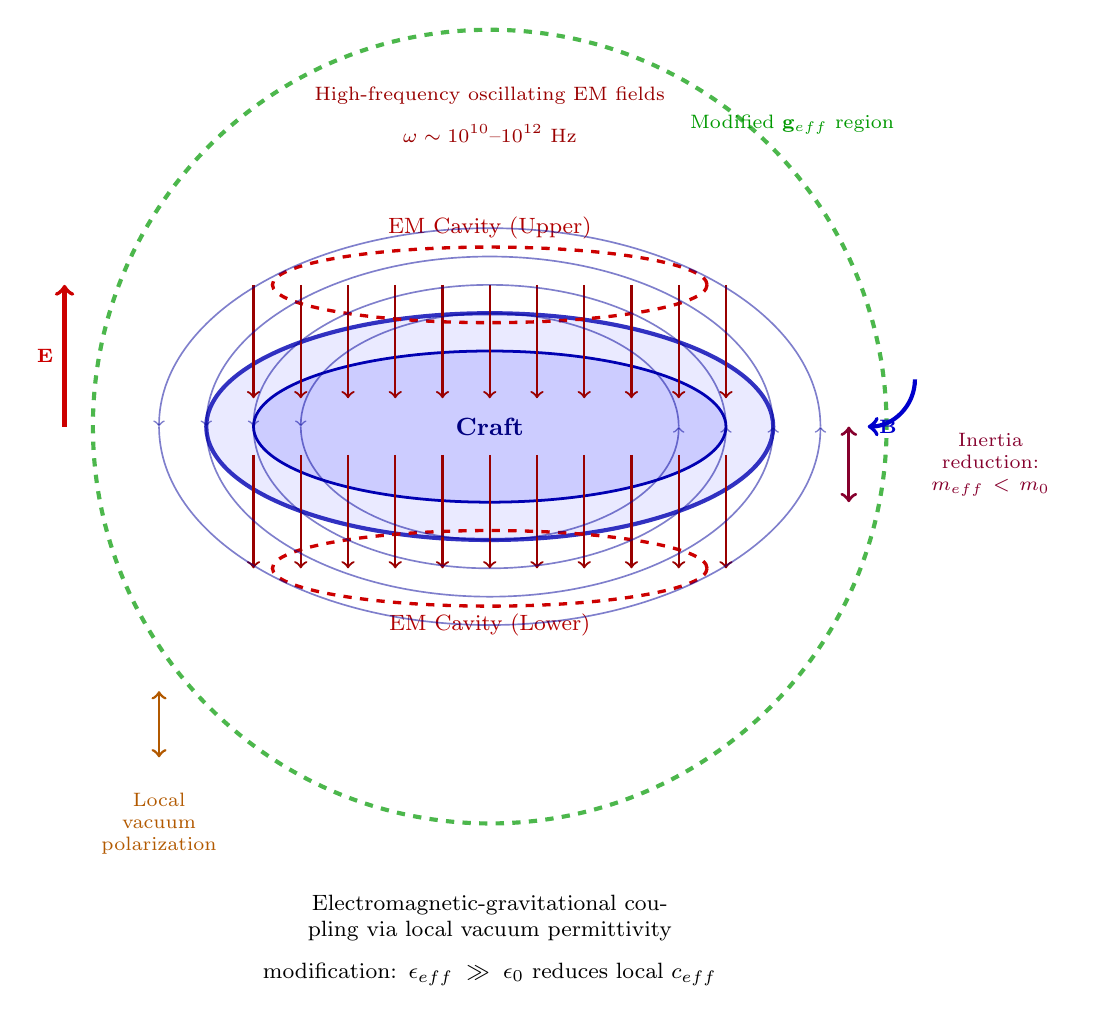
\begin{tikzpicture}[scale=1.2]

    % Craft body (diamond/disc shape)
    \begin{scope}
      \fill[blue!10!white, draw=blue!70!black, line width=1.5pt, opacity=0.8]
        (0,0) ellipse (3cm and 1.2cm);
      \fill[blue!20!white, draw=blue!70!black, line width=1pt]
        (0,0) ellipse (2.5cm and 0.8cm);
      \node[blue!50!black, font=\small\bfseries] at (0,0) {Craft};
    \end{scope}

    % Electromagnetic field generating cavity (upper)
    \draw[red!80!black, line width=1.2pt, dashed]
      (0,1.5) ellipse (2.3cm and 0.4cm);
    \node[red!70!black, font=\footnotesize] at (0,2.1) {EM Cavity (Upper)};

    % Electromagnetic field generating cavity (lower)
    \draw[red!80!black, line width=1.2pt, dashed]
      (0,-1.5) ellipse (2.3cm and 0.4cm);
    \node[red!70!black, font=\footnotesize] at (0,-2.1) {EM Cavity (Lower)};

    % Electric field lines (vertical, representing high-frequency oscillating fields)
    \foreach \x in {-2.5,-2.0,...,2.5} {
      \draw[->, red!60!black, line width=0.8pt]
        (\x,1.5) -- (\x,0.3);
      \draw[->, red!60!black, line width=0.8pt]
        (\x,-0.3) -- (\x,-1.5);
    }

    % Magnetic field lines (horizontal, circular pattern)
    \foreach \r in {2.0, 2.5, 3.0, 3.5} {
      \draw[blue!60!black, opacity=0.5, line width=0.6pt, ->]
        (\r,0) arc (0:180:\r cm and 0.6*\r cm);
      \draw[blue!60!black, opacity=0.5, line width=0.6pt, ->]
        (-\r,0) arc (180:360:\r cm and 0.6*\r cm);
    }

    % Effective gravitational field modification region (dashed circle)
    \draw[green!60!black, line width=1.5pt, dashed, opacity=0.7]
      (0,0) circle (4.2cm);
    \node[green!60!black, font=\scriptsize] at (3.2,3.2)
      {Modified $\mathbf{g}_{\text{eff}}$ region};

    % Field direction arrows and labels
    \draw[->, red!80!black, line width=1.5pt]
      (-4.5,0) -- (-4.5,1.5) node[midway, left, font=\scriptsize] {$\mathbf{E}$};
    \draw[->, blue!80!black, line width=1.5pt]
      (4.5,0.5) arc (0:-90:0.5cm) node[right, font=\scriptsize] {$\mathbf{B}$};

    % Vacuum polarization annotation
    \draw[orange!70!black, line width=1pt, <->]
      (-3.5,-3.5) -- (-3.5,-2.8);
    \node[orange!70!black, font=\scriptsize, align=center] at (-3.5,-4.2)
      {Local\\vacuum\\polarization};

    % Inertial mass reduction indicator
    \draw[purple!70!black, line width=1.2pt, <->]
      (3.8,0) -- (3.8,-0.8);
    \node[purple!70!black, font=\scriptsize, align=center, text width=2cm] at (5.3,-0.4)
      {Inertia\\reduction:\\$m_{\text{eff}} < m_0$};

    % Frequency annotation
    \node[red!60!black, font=\scriptsize, align=center] at (0,3.5)
      {High-frequency oscillating EM fields};
    \node[red!60!black, font=\scriptsize] at (0,3.1)
      {$\omega \sim 10^{10}$--$10^{12}$ Hz};

    % Physical mechanism annotation (bottom)
    \node[black, font=\footnotesize, align=center, text width=7cm] at (0,-5.2)
      {Electromagnetic-gravitational coupling via local vacuum permittivity};
    \node[black, font=\footnotesize, align=center, text width=7cm] at (0,-5.8)
      {modification: $\epsilon_{\text{eff}} \gg \epsilon_0$ reduces local $c_{\text{eff}}$};

  \end{tikzpicture}

  \caption{Schematic diagram of the Pais inertia reduction concept. High-frequency electromagnetic fields (red arrows, $\mathbf{E}$) are generated in resonant cavities above and below the craft. These fields interact with the magnetic component ($\mathbf{B}$, blue curves) to modify the local vacuum permittivity $\epsilon_{\text{eff}}$, creating a region (green dashed circle) where the effective gravitational acceleration $\mathbf{g}_{\text{eff}}$ and inertial mass $m_{\text{eff}}$ are reduced below their rest values. The mechanism relies on electromagnetic-gravitational coupling mediated by vacuum polarization, proposing that extreme field configurations can locally alter spacetime properties. Note: This represents a speculative engineering concept; experimental validation remains pending (TRL 1-2).}
  \label{fig:pais_inertia_reduction}
\end{figure}
